% ComptonScatteringSpectra
\chapter{Compton Scattering}
\label{ch:ComptonScattering}
\section{Compton Scattering}
Compton scattering is the inelastic scattering of a photon off a free charged particle, usually an electron.
The incident photon undergoes a decrease in energy, transfering the energy to the kinetic energy of the electron while also having a scattered photon.
Figure \ref{fig:ComptonScattering} is a representation of the phenoma, in which the incidnet photon has a wavelength $\lambda$ which after scattering angle $\theta$ has a final energy of $\lambda'$.
\begin{figure}
  \centering
  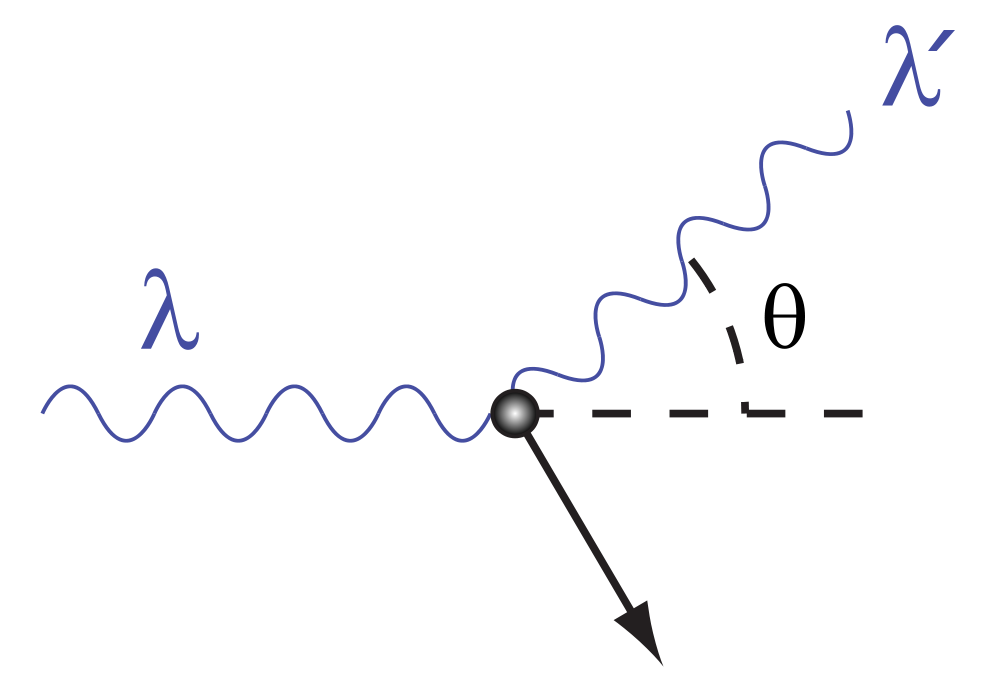
\includegraphics[width=0.45\textwidth]{ComptonScattering}
  \caption{Compton Scattering of a Photon off an Electron}
  \label{fig:ComptonScattering}
\end{figure}
The change in the energy of a compton scattered photon can be expresesed as \eqref{eqn:PhotonEnergyDiff}, where $E'$ is the final photon energy and $E$ is the initial photon energy, $m_e$ is the mass of the electron and $c$ is the speed of light.
\begin{align}
  \label{eqn:FinalPhotonEnergy}
  \frac{1}{E'} -\frac{1}{E} = \frac{1}{m_e c^2}\left(1-\cos\theta\right) 
\end{align}
Using the conservation of energy, the energy given to the electron, $E_e$ must be equal to the difference in the initial and final photon energies \eqref{eqn:EnergyElectron}
\begin{align}
  \label{eqn:EnergyElectron}
  E_e &= E - E' \\ \notag
   &= E - \frac{E m_e c^2}{m_e c^2 + E (1-\cos\theta)}
\end{align}
The probability of scattering and imparting energy is provided by the Klein-Nishina formula \eqref{eqn:KleinNishia}.
\begin{align}
  \label{eqn:KleinNishina}
  d\sigma = \frac{1}{2} r_0^2 \left(\frac{E'}{E}\right)^2 \left(\frac{E'}{E} + \frac{E}{E'}-\sin^2\theta\right)d\Omega
\end{align}
If $f(\theta)$ is defined as $f(\theta) = \frac{1}{2}\left(\frac{E'}{E}\right)^2 \left(\frac{E'}{E} + \frac{E}{E'}-\sin^2\theta\right)$ and assuming the scattering is isotropic leading to $d\Omega = \sin\theta d\theta d\phi$ it is then possible to express \eqref{eqn:KleiNishina} as \eqref{eqn:KleinNishinaShort}.
\begin{align}
  \label{eqn:KleinNishinaShort}
    d\sigma = r_0^2 f(\theta)\sin\theta d\theta d\phi
\end{align}
It is then possible to integrate over $\phi$, and then divide by the differential scattering angle to arrive at \eqref{eqn:DiffKleinNishina}.
\begin{align}
  \label{eqn:DiffKleinNishina}
  d\sigma &=\int_{\phi=0}^{2\pi} r_0^2 f(\theta)\sin\theta d\theta d\phi\\
  \frac{d\sigma}{d\theta} &=2\pi r_0^2 f(\theta)\sin\theta
\end{align}
However the probability of scattering at a given kinetic energy of the electron is desiered, $d\sigma/dE_e$.
With the chain rule and a few algebraic maniupulations it is possible to arrive at \eqref{eqn:DiffE}, and if the derivative of \eqref{eqn:EnergyElectron} is taken with respect to $\theta$ the differnetial energy scattering can be expressed as \eqref{eqn:dSdEKleinNishina}.
\begin{align}
  \label{eqn:DiffE}
  \frac{d\sigma}{dE_e} & = \frac{d\sigma}{d\theta} \frac{d\theta}{dE_e} \\
   & = \frac{d\sigma}{d\theta} \left[\frac{dE_e}{d\theta}\right]^{-1} 
\end{align}
\begin{align}
  \label{eqn:dSdEKleinNishina}
\frac{d\sigma}{dE_e} = 2\pi r_e^2 \sin \theta f(\theta)\left [ \frac{1+\frac{E}{m_e c^2}\left(1-\cos\theta \right)^2}{E^2 \sin \theta} \right ]
\end{align}

The Compton scattered spectra is plotted for \iso[60]{Co}, as shown in Figure \ref{fig:ComptonScatteredSpectra}.
\missingfigure{Compton Scattered Spectra}
%\begin{figure}
%  \caption{\iso[60]{Co} Scattered Photon Spectra}
%  \label{fig:ComptonScatteredSpectra}
%\end{figure}

\section{Computational Spectra}
The comparison of the analytical and simulated secondary electron Compton scattered sepectra can be preformed if one treats the analytical Compton scattered spectra as a probability distribution and selects from that distribution, utilizing the appropriate binning.

A rejection method was chosen in order to select from the scattering distribution, in which the probability of keeping a value was proportional to the relative value of the function evaluated at that energy.

